\chapter[Opis rozwiązania Apache Thrift][Opis rozwiązania Apache Thrift]{Opis
rozwiązania Apache Thrift}

Thrift to narzędzie, którego głównym celem jest umożliwienie tworzenia
skalowanych oraz interoperacyjnych usług. Biblioteka ta~pierwotnie została
na~otwartej licencji Apache 2.0
zaimplementowana i~była używana przez Facebooka, ale~aktualnie jest dostępna
(http://www.apache.org/licenses/LICENSE-2.0.html).

\vspace{5mm}
Thrift dzięki prostemu językowi IDL (język opisu interfejsu ang.~\emph{Interface
Definition Language}) pozwala definiować oraz tworzyć usługi dla~wielu
popularnych i~rozwijanych języków programowania. W~oparciu o~plik w~języku IDL
niezależny od~języka programowania Thrift generuje biblioteki służące
do~transportu danych pomiędzy klientem a~serwerem, wystawiając do~nich
odpowiednie interfejsy. Programista zajmuje się~jedynie implementacją
faktycznego działania aplikacji w~oderwaniu od~sposobów przekazywania danych,
co~sprawia, że~tworzenie rozwiązań w~oparciu o~RPC (zdalne wywołanie procedury,
ang.~\emph{Remote Procedure Call}) jest bardzo proste.

\section[Architektura Apache Thrift][Architektura Apache Thrift]{Architektura
Apache Thrift}
\begin{figure}[H]
\center
\flushleft
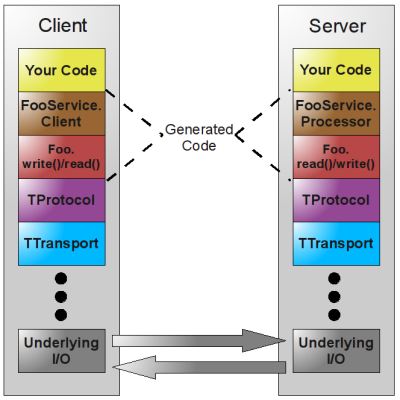
\includegraphics[keepaspectratio=true]{img/thrift_arch.png}
\caption{Źródło: http://jnb.ociweb.com/jnb/jnbJun2009.html}
\label{fig:thriftArch}
\end{figure}

\vspace{5mm}
Diagram przedstawia stos warstw implementacyjnych, które umożliwiają
komunikację RPC zgodnie z filozofią Apache Thrift.  Pierwsze trzy górne warstwy
stanowią kod napisany w tym samym języku, dla którego kompilator IDL Apache
Thrift wygenerował kod. Pierwsza warstwa to kod użytkownika-programisty, który
wykorzystuje dostarczoną abstrakcję RPC. Dwie następne warstwy to wygenerowany
kod realizujący pożądane przez użytkownika usługi. Pozostałe, niższe warstwy są
niezależne od pliku opisu interfejsu - wykorzystywany jest kod bibliotek
odpowiednich do realizacji komunikacji.

\section[Apache Thrift IDL][Apache Thrift IDL]{Apache Thrift IDL}
\hspace*{-\parindent}%
\begin{minipage}{\linewidth}
\subsection[Wspierane podstawowe typy danych][Wspierane podstawowe typy
danych]{Wspierane podstawowe typy danych}
\begin{itemize}
	\item \textbf{bool} - wartość logiczna 
	\item \textbf{byte} - bajt ze znakiem
	\item \textbf{i16} - 16 bitowa liczba całkowita ze znakiem
	\item \textbf{i32} - 32 bitowa liczba całkowita ze znakiem
	\item \textbf{i64} - 64 bitowa liczba całkowita ze znakiem
	\item \textbf{double} - 64 bitowa liczba zmienno pozycyjna
	\item \textbf{string} - tekstowy typ danych
\end{itemize}
\end{minipage}

\subsection[Kontenery][Kontenery]{Kontenery}
\hspace*{-\parindent}%
\begin{minipage}{\linewidth}
Thrift umożliwia definiowanie zbiorów danych przy pomocy trzech rodzajów
kontenerów:
\begin{itemize}
	\item \textbf{list}<typ> - uporządkowana kolekcja 
	\item \textbf{set}<typ> - nieuporządkowana kolekcja
	\item \textbf{map}<typ\_klucza, typ\_wartości>  - mapa
	klucz-wartość
\end{itemize}
\end{minipage}

\subsection[Struktury][Struktury]{Struktury}
Thrift umożliwa definiowanie złożonych struktur danych przypominających
struktury z języka C. Definiuje się je w następujący sposób:
\begin{lstlisting}[language=C, style=incode]
struct <nazwa_struktury>
{
	1:<typ_danych_1> <nazwa_skladowej_1>,
	2:<typ_danych_2> <nazwa_skladowej_2>,
	3:<typ_danych_3> <nazwa_skladowej_3>,
}
\end{lstlisting}

\subsection[Wyjątki][Wyjątki]{Wyjątki}
Deklarowanie wyjątków jest podobne do~definiowania struktur.

\begin{lstlisting}[language=C, style=incode, morekeywords={exception}]
exception <nazwa_wyjatku>
{
	1:<typ_danych_1> <nazwa_skladowej_1>,
	2:<typ_danych_2> <nazwa_skladowej_2>,
	3:<typ_danych_3> <nazwa_skladowej_3>,
}
\end{lstlisting}

\newpage
\section[Zalety korzystania z rozwiązania Apache Thrift][Zalety korzystania z
rozwiązania Apache Thrift]{Zalety korzystania z rozwiązania Apache Thrift}
Wykorzystanie Apache Thrift posiada wiele zalet z~perspektywy programisty:
\begin{itemize}
  \item posiada czytelny dla~człowieka, niezależny od~języka plik opisu
  interfejsu,
  \item umożliwia zmianę protokołu i~sposobu transportu danych bez~poważnych
  zmian w~kodzie - wykorzystywane są~możliwości narzędzia Apache Thrift,
  \item zapewnia wysoką wydajność serializacji pomiędzy różnymi językami
  (w~porównaniu do~popularnych protokołów wykorzystujących XML lub~JSON) przez
  możliwość wykorzystania protokołu binarnego,
  \item serwer wielowątkowy (lub~jednowątkowy), wykorzystujący funkcje blokujące
  lub~nieblokujące dostępny ,,prosto z pudełka''.
\end{itemize}

